\documentclass{gqtekspec}
%%%%%%%%%%%%%%%%%%%%%%%%%%%%%%%%%%%%%%%%%%%%%%%%%%%%%%%%%%%%%%%%%%%%%%%%%%%%%%%%
%%
%% Filename: 	spec.tex
%%
%% Project:	CMod S6 System on a Chip, ZipCPU demonstration project
%%
%% Purpose:	
%%
%% Creator:	Dan Gisselquist, Ph.D.
%%		Gisselquist Technology, LLC
%%
%%%%%%%%%%%%%%%%%%%%%%%%%%%%%%%%%%%%%%%%%%%%%%%%%%%%%%%%%%%%%%%%%%%%%%%%%%%%%%%%
%%
%% Copyright (C) 2015-2016, Gisselquist Technology, LLC
%%
%% This program is free software (firmware): you can redistribute it and/or
%% modify it under the terms of  the GNU General Public License as published
%% by the Free Software Foundation, either version 3 of the License, or (at
%% your option) any later version.
%%
%% This program is distributed in the hope that it will be useful, but WITHOUT
%% ANY WARRANTY; without even the implied warranty of MERCHANTIBILITY or
%% FITNESS FOR A PARTICULAR PURPOSE.  See the GNU General Public License
%% for more details.
%%
%% You should have received a copy of the GNU General Public License along
%% with this program.  (It's in the $(ROOT)/doc directory, run make with no
%% target there if the PDF file isn't present.)  If not, see
%% <http://www.gnu.org/licenses/> for a copy.
%%
%% License:	GPL, v3, as defined and found on www.gnu.org,
%%		http://www.gnu.org/licenses/gpl.html
%%
%%
%%%%%%%%%%%%%%%%%%%%%%%%%%%%%%%%%%%%%%%%%%%%%%%%%%%%%%%%%%%%%%%%%%%%%%%%%%%%%%%%
%%
%%
\usepackage{import}
\usepackage{bytefield}
\project{CMod S6 SoC}
\title{Specification}
\author{Dan Gisselquist, Ph.D.}
\email{dgisselq (at) opencores.org}
\revision{Rev.~0.3}
\begin{document}
\pagestyle{gqtekspecplain}
\titlepage
\begin{license}
Copyright (C) \theyear\today, Gisselquist Technology, LLC

This project is free software (firmware): you can redistribute it and/or
modify it under the terms of  the GNU General Public License as published
by the Free Software Foundation, either version 3 of the License, or (at
your option) any later version.

This program is distributed in the hope that it will be useful, but WITHOUT
ANY WARRANTY; without even the implied warranty of MERCHANTIBILITY or
FITNESS FOR A PARTICULAR PURPOSE.  See the GNU General Public License
for more details.

You should have received a copy of the GNU General Public License along
with this program.  If not, see \texttt{http://www.gnu.org/licenses/} for a copy.
\end{license}
\begin{revisionhistory}
0.3 & 5/23/2016 & Gisselquist & Draft for comment, includes ZipOS and PMod
		pin mapping\\\hline
0.2 & 5/14/2016 & Gisselquist & Updated Draft, still not complete \\\hline
0.1 & 4/22/2016 & Gisselquist & First Draft \\\hline
\end{revisionhistory}
% Revision History
% Table of Contents, named Contents
\tableofcontents
\listoffigures
\listoftables
\begin{preface}
The Zip CPU was built with the express purpose of being an area optimized,
32--bit FPGA soft processor.  

The S6~SoC is designed to prove that the Zip~CPU has met this goal.

There are two side--effects to this.  First, the project proves how capable a
CMod--S6 is, and second, this project provides demonstration implementations
of how to interact with a variety of PMod devices: the audio amplifier, 
the serial 2--line LCD display, the USBUART, and the 16--character numeric
keypad.
\end{preface}

\chapter{Introduction}
\pagenumbering{arabic}
\setcounter{page}{1}

% What is old
The Zip~CPU is a soft core CPU designed to fit within an FPGA, to use a minimum
amount of the FPGA's resources, and yet to provide the services of a fully
capable 32--bit computer.  It is based upon a Von~Neumann architecure and so a 
single 32--bit wishbone bus provides it with access to both peripherals and
memory.

% What does the old lack?
Previous demonstrations of the Zip~CPU have focused on larger FPGAs, such as
the Spartan--6 LX9 and LX25 and the Artix--7 35T.  On these FPGA's,
the Zip~CPU runs in a pipelined configuration where it is tightly integrated
with a prefetch/instruction cache.  While these demonstrations have shown that
the Zip~CPU can act as a very simple CPU in these environments, they really
haven't demonstrated the ability of the Zip~CPU to use only a minimum amount
of the FPGA's resources.

% What is new
The CMod~S6 board provides the opportunity for that demonstration rather nicely.
% What does the new have that the old lacks
\begin{enumerate}
\item The Spartan--6 LX4 FPGA is very limited in its resources: 
	It only has 2,400 look--up tables (LUTs), and can only support 
	a 4,096~Word RAM memory (16 kB).
\item With only 4kW RAM, the majority of any program will need to be placed into
	and run from flash. 
\item While the chip has enough area for the CPU, it doesn't have enough area
	to include the CPU and \ldots write access to the flash, debug access,
	wishbone command access from the UART, pipelined CPU operations,
	a prefetch cache and more.  Other solutions will need to be found.
\end{enumerate}

Of course, if someone just wants the functionality of a small, cheap, CPU,
this project does not fit that role very well.  While the S6 is not very
expensive at nearly \$70, it is still an order of magnitude greater than it's
CPU competitors in price.  This includes such CPU's as the Raspberry Pi Zero
(\$5), or even the TeensyLC (\$12).

% What performance gain can be expected?

If, on the other hand, what you want is a small, cheap, CPU that can be
embedded within an FPGA without using too much of the FPGA's resources, this
project will demonstrate that possibility as well as some utility. 
Alternatively, if you wish to study how to get a CPU to work in a small,
constrained environment, this project may be what you are looking for.

Finally, because the Zip~CPU and the included ZipOS are as small and simple as
they are, the code base found here will be simpler to understand than the
code bases for some of these other projects.  For example, the Zip~CPU
instruction set is very simple.  With less than 40 instructions, it is much
easier to understand and learn than the ARM instruction set.  Further, unlike
the ARM, the entire specification for and description of the Zip~CPU is
publicly available.  Likewise, an operating system such as the ZipOS that has
less than \hbox{3,000} lines of code will be much easier to understand than any
Linux operating system--even if it has much less functionality.

\chapter{Architecture}
Fig.~\ref{fig:architecture}
\begin{figure}\begin{center}
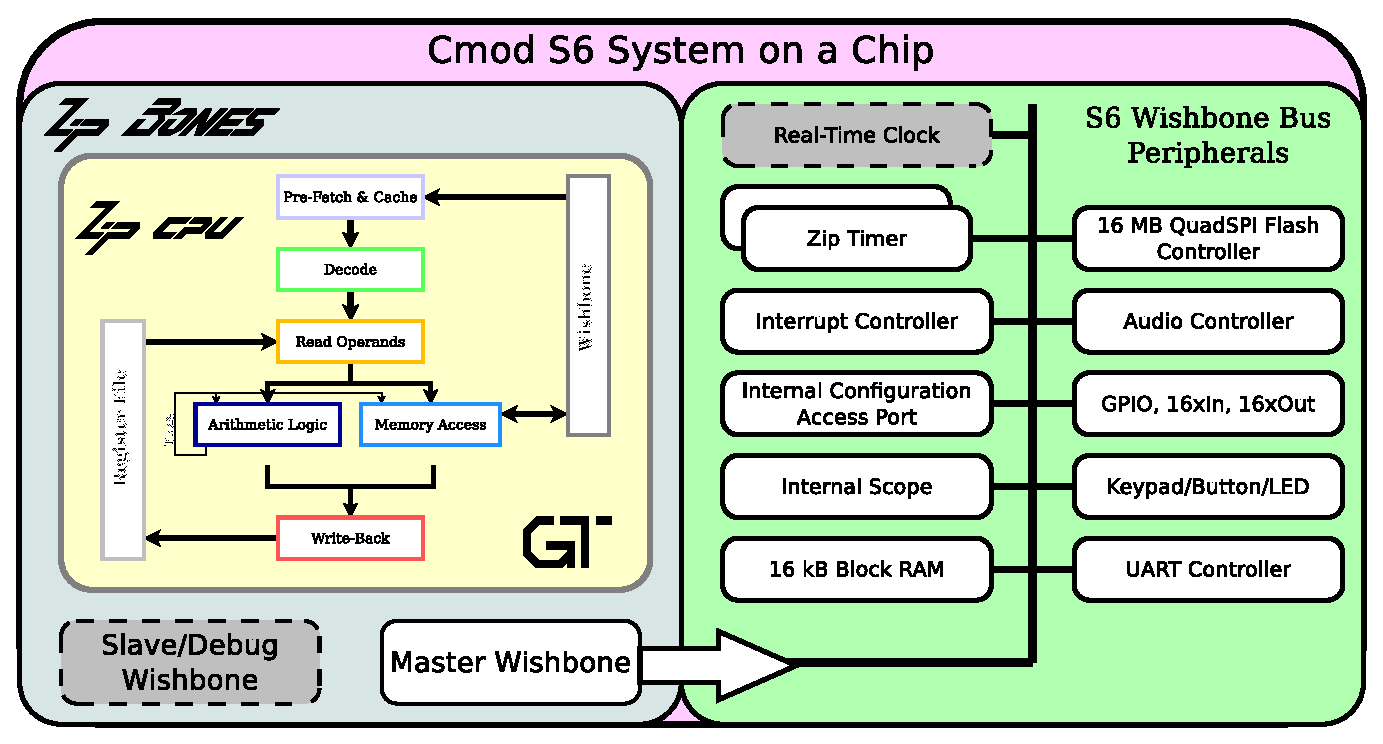
\includegraphics[width=5in]{../gfx/s6bones.eps}
\caption{CMod S6 SoC Architecture: Zip~CPU and
	Peripherals}\label{fig:architecture}
\end{center}\end{figure}
shows the basic internal architecture of the S6~SoC.  In summary, it consists
of a CPU
coupled with a variety of peripherals for the purpose of controlling the
external peripherals of the S6~SoC: flash, LEDs, buttons, and GPIO.  External
devices may also be added on, and have been added on as part of this project,
such as an audio device, an external serial port, an external keypad, and an
external display.  All of these devices are then available for the CPU to
interact with.

If you are familiar with the Zip CPU, you'll notice this architecture provides
no access to the Zip CPU debug port.  There simply wasn't enough room on the
device.  Debugging the Zip~CPU will instead need to take place via other means,
such as dumping all registers and/or memory to the serial port on any reboot.

Further, the Zip~CPU has no ability to write to flash memory.  For this reason,
there exists an alternate CMod S6~SoC architecture, shown in
Fig.~\ref{fig:altarchitecture}.
\begin{figure}\begin{center}
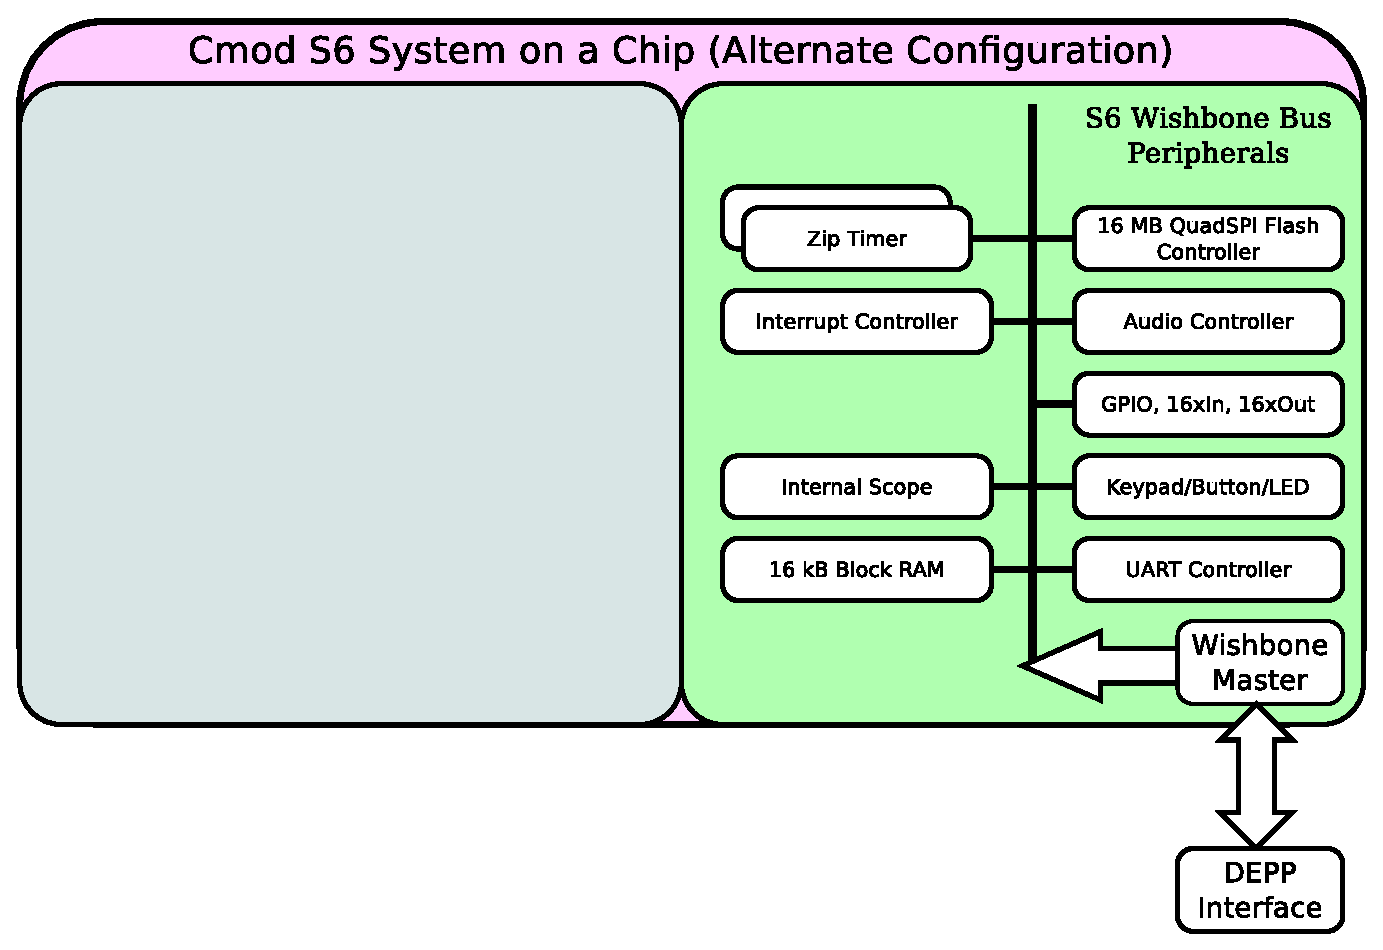
\includegraphics[width=5in]{../gfx/altbones.eps}
\caption{Alternate CMod S6 SoC Architecture: Peripherals, with no
	CPU}\label{fig:altarchitecture}
\end{center}\end{figure}
Using this alternate architecture, it should be possible to test the peripherals
and program the flash memory.  Both architectures may be loaded into the flash,
together with the programming code for the Zip CPU.

The basic approach to loading the board is actually quite simple.  Using the
Digilent ADEPT JTAG configuration program, {\tt djtgcfg}, the alternate 
configuration may be written directly to the device.  Once this alternate
configuration has been loaded, the flash may be examined and programmed using
the {\tt zipload} utility.  This utility uses Digilent's Asynchronous Parallel
Port interface (DEPP) to communicate with the device, and in particular to 
tell the device what to write to the flash.  When writing to the flash,
the {\tt zipload} utility will program both a primary and an alternate
FPGA configuration into the configuration section of the flash, as well as
computer code into the rest of the flash.  Once complete, the system may then be
reloaded with the primary configuration file which will contain an image of
the CPU.  The CPU will then begin following the instructions found in flash
memory.


\chapter{Software}
This chapter provides an overview of the software that is available to support
the S6~SoC.  This includes not only the RTL, the Makefiles, and the software
that will run on the Zip~CPU within the S6~SoC, but also the support software
necessary for communicating with the S6~SoC in its alternate configuration.

\section{Directory Structure}
\begin{itemize}
\item[{\tt trunk/bench}] Contains software for emulating the S6 without the S6
	present.
  \begin{itemize}
	\item[{\tt trunk/bench/cpp}]  All of the bench testing software is
		written in C++, so it is found in this directory.  Primary
		among these programs is the {\tt zip\_sim} program which will
		simulate the Zip~CPU within the S6~SoC.  Specifically, it
		simulates everything at or below the {\tt busmaster.v} level.

		Some, although not all, of the peripherals have been simulated
		and made a part of this simulation.  These include the
		Quad--SPI flash, the UART, and the LED's.

  \end{itemize}
\item[{\tt trunk/doc}] All of the documentation for the S6~SoC project may be
	found in this documentation directory.  Specifically, I would commend
	your attention to anything with a {\tt .pdf} extension, as these
	are the completed documents.  Among these you should find a copy of the
	GPL copyright under which this software is released, as well as a 
	pre--built copy of this document.
  \begin{itemize}
	\item[{\tt trunk/doc/gfx}] Here is where the graphics are located in
		support of this specification document.
	\item[{\tt trunk/doc/src}] And here is where the \LaTeX files are
		kept that were used in building both this document as well as
		the GPL copyright.
  \end{itemize}
\item[{\tt trunk/rtl}] Verilog files.  The two top--level files are
	{\tt toplevel.v} for the primary top level module, and
	{\tt alttop.v} for the alternate load.
  \begin{itemize}
	\item[{\tt trunk/rtl/cpu}]	Verilog files containing the Zip~CPU
		core and peripherals.  The toplevel file here is the
		{\tt zipbones.v} file, although some of the peripherals, such
		as the {\tt ziptimer.v} are referenced independently.
  \end{itemize}
\item[{\tt trunk/sw}] The main software directory, primarily a repository
	for software subdirectories beneath it.
  \begin{itemize}
	\item[{\tt trunk/sw/dev}]  This directory holds a variety of 
		simple programs for the Zip~CPU, such as {\tt helloworld},
		{\tt doorbell} and {\tt doorbell2}, as well as software drivers
		for various peripherals, such as the real--time clock simulator,
		and the keypad and display device drivers.
	\item[{\tt trunk/sw/host}]  This directory holds support software which
		can be built on and run on the host machine.  Building this
		software will involve adjusting the Makefile so that it knows
		where your local ADEPT installation directory is.\footnote{Many
		of the programs also depend upon the serial number of my CMod
		S6 device.  This will need to be adjusted in any new install.}
		Once built, you will find a variety of very useful programs
		within here. 
	\item[{\tt trunk/sw/zipos}]  This directory contains the source code for
			a rudimentary, very basic, operating system that I
			call the ZipOS. 
  \end{itemize}
\end{itemize}

\section{Zip CPU Tool Chain}
To build programs for the Zip~CPU, you will need the Zip~CPU toolchain.  You
can find this as part of the Zip~CPU project, available at OpenCores.  Building
the Zip~CPU project should result in a set of binaries in the
\hbox{\tt zipcpu/trunk/sw/install/cross-tools/bin} directory.  Make this
directory a part of your path, and you should be able to build the CMod S6
Zip~CPU software.  Specifically, you will need to use {\tt zip-gcc},
{\tt zip-as}, {\tt zip-ld}, and {\tt zip-cpp}.  Other tools, such as
{\tt zip-objdump} and {\tt zip-readelf}, may also prove to be very useful when
trying to figure out what is going on within the SoC.

\section{Bench Test Software}

Bench testing software currently consists of the {\tt zip\_sim} program found
within {\tt trunk/bench/cpp}.  This program requires Verilator to run, and
simulates in a cycle accurate fashion, the entire S6~SoC from {\tt busmaster.v}
on down.  Further, the external Quad--SPI flash memory, UART, and LED's are
also simulated, although the 2--line display, audio, and keypad are not.

\section{Host Software}
Several software programs have been built to support the S6~SoC from a nearby
host.  These programs include:
\begin{itemize}
\item {\tt dumpuart}: My current approach to debugging involves
	dumping the state of the registers and memory to the
	UART upon reboot.  The dumpuart command found here is
	designed to make certain that the UART is first set
	up correctly at 9600~Baud, and second that everything
	read from the UART is directly sent to both a file and
	to the screen.  In this fashion, it is similar to the
	UNIX {\tt tee} program, save for its serial port
	attachment.
\item {\tt readflash}: As I am loathe to remove anything from
	a device that came factory installed, the
	{\tt readflash} program reads the original installed
	configuration from the flash and dumps it to a file.

	This program is only useful when the alternate configuration is loaded.

\item {\tt wbregs}: This program offers a capability very similar to the 
	PEEK and POKE capability Apple user's may remember from before the
	days of Macintosh.  {\tt wbregs <address>} will read from the
	Wishbone bus the value at the given address.  Likewise
	{\tt wbregs <address> <value>} will write the given value into the
	given address.  While both address and value have the semantics of
	numbers acceptable to {\tt strtoul()}, the address can also be a named
	address.  Supported names can be found in {\tt regdefs.cpp}, and their
	register mapping in {\tt regdefs.h}.

	As examples, {\tt wbregs version}, will return the build date, or
	version of the RTL.  {\tt wbregs spio} reads the special purpose
	I/O register, and {\tt wbregs gpio 0xffffffff} will set all output
	GPIO ports high while {\tt wbregs gpio 0xffff0000} will set all 
	output GPIO ports to ground.

	This program is only useful when the alternate configuration is loaded.

\item {\tt zipload}: This is the primary program you will need to get your
	software loaded on the CMod.  It takes three arguments.  The first is
	the name of the primary Xilinx configuration file, the second is the
	name of an alternate Xilinx configuration file, and the third is the
	name of the Zip~CPU program you wish to write to Flash memory.

	Each of these arguments is optional.  For example, if only one
	configuration file is given, the loader will load the primary
	configuration.  If only one Zip~CPU program is given, the program will
	be loaded into the program memory area and the configuration file areas
	will be left untouched.

	This program is only useful when the alternate configuration is loaded.
\end{itemize}
\section{Zip CPU Programs}
The following are a list of simple, independent, single-task example programs
that will run on the S6~SoC:
\begin{itemize}
\item {\tt helloworld}: The first program any programmer should build,
	``Hello, world!''  This program sends the string, ``Hello, world!''
	over the UART connection once per second.  It is a very valuable
	program because, if you can get this program running, you know you have
	a lot of things working and working correctly.  For example, running
	this program means you can run the {\tt zip-gcc} compiler, load
	the auxiliar configuration, load the program info flash memory, load
	the primary configuration, and read from the UART port.  It also means
	that you must have the UART port properly configured and wired to your
	CMod board.
\item {\tt doorbell}: This annoying program verifies the functionality of the
	audio device by playing a doorbell sound to the audio port.  It will
	then wait ten seconds, and play the doorbell sound again (and again,
	and again).  (It gets old after a while ...)
\item {\tt doorbell2}: This adds to the functionality of the {\tt doorbell}
	program a wait for keypress, and a display of the current time on the
	2--line display.  While almost our fully functional program, this
	does not include any menus to configure the device or set time, since
	it doesn't include any keypad functionality.
\item {\tt kptest}: A test of whether or not they keypad driver works.  When
	run, anytime a key is pressed, the key's associated printable character
	will be sent to the UART.  Further, pressing an `F' on the keypad will
	also send a newline over the UART, in case you wish to keep your lines
	from getting too long.
\end{itemize}
\section{ZipOS}
The ZipOS is a brand new operating system, specifically designed to run on the
ZipCPU.  It is both pre--emptive and multitasking, although with many
limitations.  Those familiar with the internals of other operating systems, such
as Linux, may laugh that I call this an Operating System at all: it has no
memory management unit, no paging, no virtual memory, no file I/O access, no
network stack, no ability to dynamically add or remove tasks, indeed it hardly
has any of the things most often associated with an Operating System.  It does,
however, handle interrupts, support multiple pre--emptive tasks in a
multitasking, timesharing fashion, and it supports some very basic and
rudimentary system calls.  In a similar fashion, it does contain just about all
of the functionality necessary for a multi--tasking microcontroller built
around a do--forever loop.  For its size, I consider it an impressive
achievement.  You are welcome to disagree with me, however.

This version of the ZipOS starts in the {\tt resetdump.s} code, so that upon
any startup the ZipOS will dump register contents, the BusError register, and
any scope contents to the UART.  This can take some time, so you may wish to
configure what you really wish to send--if anything.  If desired,
{\tt resetdump} can also be configured to also dump the entire memory as well
while only using 9~memory locations.  All of this is quite useful in case the
Zip~CPU encounters a bus error or other sort of error that causes it to hang,
stall, or reboot, as the CPU registers are very carefully not touched prior to
being sent to the UART output port.  This extends to all registers save the
supervisor PC and CC registers, which would've been reset by a reboot anyway.

{\tt resetdump.s} then calls a rudimentary bootloader, to load the parts of
the ZipOS that need to run faster into Block RAM.  The choice of what parts
to load into Block RAM is made on a file by file basis, and found within
the linker script, {\tt cmodram.ld}.

Upon completion, {\tt resetdump.s} calls the entry routine for the O/S,
{\tt kernel\_entry()} found in {\tt kernel.c}.  This is the main task loop for
the entire O/S, and worth studying if you are interested in understanding how
the O/S works.

The user tasks are found (mostly) within {\tt doorbell.c}, also found in the
ZipOS directory.  This file contains two kernel entry points, {\tt kntasks()},
which returns the number of user tasks the kernel needs to know about, and
{\tt kinit()}, which builds each of the tasks and connects their file 
descriptors to the various devices they will be referencing.
\subsection{System Calls}
The ZipOS supports a variety of system calls, listed here:
\begin{itemize}
\item {\tt int wait(unsigned event\_mask, int timeout)}

	Halts the execution of a process until an event matching the
	{\tt event\_mask} takes place, or a {\tt timeout} (in milliseconds)
	has been reached.  The events that can take place are a
	bitmask of the various interrupts the CPU supports, together with a 
	bitmask of the software interrupt values found in {\tt swint.h}.

	The {\tt timeout} value can either be zero, to return immediately with
	the list of events that have taken place, negative, to wait
	indefinitely, or a positive number of milliseconds in order to wait at
	least that time for the event of interest to take place.

	Waiting on a zero event mask allows a process to sleep for any number
	of requested milliseconds.

	When wait returns, any events returned by the wait have been cleared.

	The other thing to be aware of is that events may accumulate before the
	wait system call.  Nothing within the wait system call clears prior
	events.  These prior events be returned and cleared, though, if
	the wait call indicates an interest in those events.  

	Upon return, the a bitmask of events that have taken place will be
	returned to the process.

\item {\tt int clear(unsigned event\_mask, int timeout)}

	This system call works closely with the wait system call.  Indeed,
	when the timeout given is zero, the two function nearly identically. 
	It clears any of the requested events which may be pending, and returns
	a bit mask of the events that were pending and cleared.

	However, if the timeout is given (and is positive), then {\tt clear()}
	starts a timer.  Once the timer has completed, a timeout event,
	{\tt SWINT\_TIMEOUT}, will be generated and made available to the task
	to wait upon it.

	In a similar fashion, if the timeout is negative, then any pending
	timeout is cleared.

\item {\tt void post(unsigned event\_mask)}

	Certain devices, such as the real--time clock and the doorbell
	reader, need the ability of being able to post events to any listener
	within the O/S.  The POST system call allows them to POST events in
	this manner.

	Were the ZipOS to be closer to a secure O/S, it might restrict what
	events each process could post.  Right now, however, any process can
	post any event--whether it be a hardware or a software generated event.

\item {\tt void yield(void) }

	This is simply a way of being nice to other processes.  This system
	call takes no arguments and simply asks the scheduler to schedule the
	next process.  It does not take this process off of the ready to run
	list, so the next process may be this one.  However, since the scheduler
	is a round--robin scheduler, it will only return to this process once
	it has gone through all other available processes checking whether or
	not they are available to be run.

\item {\tt int read(int fid, void *buf, int len)}

	This is roughly the same system call as the POSIX read() system
	call.  It reads some number of words (not octets) from the file
	descriptor (device) specified by {\tt fid} into the memory address
	range starting at {\tt buf} and {\tt len} words long.  If the memory
	requested is unavailable,
	the read will wait until it is available, possibly indefinitely.

	Upon return, the {\tt read()} function call returns the number of
	words actually read, or a negative value on error.

	As a future feature, a {\tt read()} system call should be able to be
	interrupted by a timeout.  This feature has not (yet) been implemented,
	but will likely be implemented via a combination of the {\tt clear()}
	system calls ability to set timeouts together with the {\tt read()}
	functions ability to wait for available data.

\item {\tt int write(int fid, void *buf, int len)}

	This is roughly the same system call as the POSIX {\tt write()} system
	call.  It writes some number of memory addresses (words, not octets),
	to the given file descriptor.  If there is no reader task or device
	associated with the file descriptor, then the {\tt write()} system
	call will block forever once the internal pipe fills up.  Otherwise,
	if something is reading from the file descriptor's pipe, the writing
	task will only stall until the data is either written to the receiving
	task, or copied into a memory buffer.

	Upon return, the {\tt write()} system call returns the number of words
	actually written to the system pipe (not necessarily the number that
	have been read), or a negative value on error.

\item {\tt unsigned time(void) }

	Returns the number of seconds since startup.  Eventually, this will
	return the number of seconds since January 1, 1970, and be identical
	to the UNIX system time() command, but that may not happen on this
	project.

% \item SEMGET
% \item SEMPUT

\item {\tt void *malloc(void)}

	Allocates memory from the system/kernel heap.  This is a very low
	overhead memory allocator that, while it does allocate memory, cannot
	free it later.  It is nearly 100\% efficient since only one memory
	address, the top of the heap, is used to determine what memory has
	been allocated.

\item {\tt void free(void *buf)}

	This function is a do--nothing stub.

\end{itemize}
\subsection{Scheduler}
The ZipOS currently supports only a round--robin scheduler.  Tasks are executed
in the order they were created, as long as they are available to be executed.
If no tasks are available to be run, the Scheduler will run the idle task which
puts the CPU to sleep while waiting for an interrupt.

\chapter{Operation}
The {\tt doorbell} program has been built to illustrate the operation of both
the Zip~CPU, the ZipOS, as well as showing off how all of the various
peripherals work.  It was envisioned after my family and I experienced an 
unexpected visitor during the wee hours of the morning.  The {\tt doorbell}
program is designed to couple the doorbell and the exterior lights to a 
single button.  Hence, when the doorbell to the house is pressed, the exterior
light is turned on for a half an hour.  This, then, would make it difficult
for someone to see inside during this time.

This chapter will present an example of how the {\tt doorbell} program works.

To run the {\tt doorbell} program, you will first need to build the various
RTL and software support programs just to get the {\tt doorbell} program on
the device:
\begin{enumerate}
\item First build the primary and alternate .bit files by building 
	with {\tt toplevel.v} and then {\tt alttop.v} as your top--level
	RTL files.  I like to place my Xilinx work directoy into
	{\tt trunk/xilinx}, and if you do the same the load scripts that
	are referenced next will work.

	Before going on, double check that both configuration .bit files were
	created, that they each fit within the device (there would be errors
	if they did not), and that they met their respective timing
	requirements.

\item Then, load the alternate bit file into the S6~SoC.  You will need
	the Digilent tools installed in order to do this.  Having done so,
	you may run {\tt make axload} from the {\tt trunk/} directory.
	If you didn't run the Xilinx ISE from within {\tt tunk/xilinx},
	you may need to find your .bit files and adjust where they load
	from, but this should be fairly straight--forward from the instructions
	within the Makefile.
\item Build the software found in the host directory.  This sotware depends
	upon Digilent's ADEPT toolsuite, so you will need to adjust the
	Makefile so that it references the toolsuite.

	{\em Note:} Currently, the host software is serial--number locked to
	my own CMod--S6.  Until I fix this and make it more user friendly,
	you'll want to switch your software to reference your own CMod.
	To do this, look for the {\tt "SN:\ldots"} lines within the `*.cpp'
	files.  Currently, there is one such line within wbregs, another
	within readflash, and the last within zipload.  To find our your own
	device's serial number, type {\tt djtgcfg enum}.  It should find one
	(or more) CMod devices connected to your system, and list each of
	their serial numbers.

	Once you've done this, you should have a working set of host support
	programs: readflash, wbregs, and zipload.

\item Using {\tt wbregs}, you may now test your configuration.  {\tt wbregs}
	works like the peek and poke programs from a generation ago. 
	{\tt wbregs <address>} will return the value of the memory (or
	peripheral) found at the {\tt <address>}.  Some addresses have names,
	such as {\tt UART}, {\tt SPIO}, {\tt GPIO}, {\tt PIC}, and so forth. 
	These names are found in {\tt trunk/sw/host/regdefs.cpp}, and their
	mappings in {\tt trunk/sw/host/regdefs.h}.

	As examples, if you type {\tt wbregs version} you should be able
	to read the version (a.k.a. build date) from the currently installed
	.bit file.  Likewise if you type {\tt wbregs uart 65}, you should see
	an `A' (i.e. a 65) sent from the S6~SoC over the serial port. 
	{\tt wbregs uart} by itself will read a single character from the
	serial port and so on.

	You should be able to test all of your peripherals by hand using
	{\tt wbregs}: GPIO, Flash, UART, keypad, buttons, LEDs, Interrupt
	controller, timer, etc.\footnote{The display and audio devices may be
	more difficult since these require multiple interactions over the
	course of a short period of time to work.}  This should give you some
	confidence in how these peripherals work, should you need it.  You
	may also use this time to verify that your wiring is properly set up.

\item If you wish to make certain you keep track of the original Flash bitfile
	that came with your device, you may read it out using {\tt readflash}.
	This will dump the contents of you flash onto {\tt qspiflash.bin}.
	You may then wish to change the name of this file, lest you overwrite
	it by running {\tt readflash} again later.

\item At this point, it's time to build the programs for the Zip~CPU.  To do
	this, you will first need to download the Zip~CPU project.  When 
	building that project, it will create a directory of programs
	(including its compiler) in
	{\tt zipcpu/trunk/sw/install/cross-tools/bin}. 
	Include this directory into your path.

\item Change into {\tt trunk/sw/dev} to build some device testing files.
	{\tt make} by itself should build some of these.

	You should now be ready to run some basic tests on the S6~SoC.

\item Let's test the UART first: back out to the main directory {\tt trunk/},
	and run\break
	{\tt sw/host/zipload sw/dev/helloworld} and then {\tt make xload}.
	Now, examine your UART port.  (You do have the PModUSBUART installed
	and connected, right?)  You should see ``Hello, world!'' printed
	over and over again once each second.

\item You may try other test files in a similar manner, such as 
	{\tt trunk/sw/dev/doorbell} and\break
	{\tt trunk/sw/dev/doorbell2}.  The first of these will just play the
	doorbell over and over again, whereas the second one will wait for a 
	button press before playing the doorbell sound.

\item Now let's go and build the ZipOS together with it's user files.  To do
	this, enter into the {\tt trunk/sw/zipos} directory and type
	{\tt make}.  If all goes well, you should now have a program named
	{\tt trunk/sw/zipos/doorbell} which you can load into your S6~SoC as
	well.

\item A final load, and we'll be done.  To do this, make {\tt axload} again,
	and this time {\tt sw/host/zipload xilinx/toplevel.bit sw/zipos/doorbell}.
	When you power on your device the next time, or after you 
	{\tt make xload}, you'll find the ZipOS running on the Zip~CPU.

\item To test the doorbell, press one of the buttons.  You should hear a
	doorbell coming out of the PModAMP2 audio port.

\item You should also be able to read the time on the LCD display.  It will be
	the wrong time (the number of seconds since power on \ldots).  To set
	the correct time, press `A' on the keypad and then type in the 6--digit
	time: HHMMSS.

	If you make a mistake, the `C' key can be used for a backspace.

\item You can also set the time of ``dawn'' by pressing a `B' on the keypad
	and then typing in the time ``dawn'' should be at.  The same is
	true for dusk, only you'll need to start that by pressing a `C' on the
	keypad.

\item Now, when the doorbell rings, the LCD will show the time the doorbell
	was pressed.  If the time is at night, the ourdoor light (oops, I
	mean LED\#3) will turn on for a half an hour (currently set to
	30~seconds, since I don't have the patience to wait a half hour while
	testing).
\end{enumerate}

Now that you've made it this far, you can go back and examine what was done
along the way, and perhaps even modify it for your own personal application.

\chapter{Registers}
There are several address regions on the S6~SoC, as shown in
Tbl.~\ref{tbl:memregions}.
\begin{table}[htbp]
\begin{center}\begin{tabular}{|p{0.75in}|p{0.75in}|p{0.5in}|p{3.0in}|}\hline
\rowcolor[gray]{0.85} Start & End & & Purpose \\\hline\hline
\scalebox{0.9}{\tt 0x000100} & \scalebox{0.9}{\tt 0x000107} & R/W & Peripheral I/O Control \\\hline
\scalebox{0.9}{\tt 0x000200} & \scalebox{0.9}{\tt 0x000201} & R/(W) & Debugging scope\\\hline
\scalebox{0.9}{\tt 0x000400} & \scalebox{0.9}{\tt 0x00043f} & R/W & Internal Configuration Access Port\\\hline
\scalebox{0.9}{\tt 0x000800} & \scalebox{0.9}{\tt 0x000803} & R/W & RTC Clock (if present)\\\hline
\scalebox{0.9}{\tt 0x002000} & \scalebox{0.9}{\tt 0x002fff} & R/W & 16kB On-Chip Block RAM \\\hline
\scalebox{0.9}{\tt 0x400000} & \scalebox{0.9}{\tt 0x7fffff} & R & 16~MB SPI Flash memory\\\hline
\end{tabular}
\caption{Address Regions}\label{tbl:memregions}
\end{center}\end{table}
In general, the address regions that are made up of RAM or flash act like
memory.  The RAM can be read and written, and the flash acts like read only
memory.\footnote{The Flash can be written, but only by an external command
while in the alternate configuration.}

This isn't quite true with the other address regions.  Accessing the I/O
region, while it will act like a memory, it may also have side-effects.  For
example, reading from the debugging scope device's data port will read a word
from the scope's buffer and advance the buffer pointer.  (More on that later.)

Finally, to keep the address decoder simple, many of these addresses are 
multiply mapped.  Hence you may find the I/O peripherals mapped throughout the
{\tt 0x0100}--{\tt 0x01ff} address region.  Other memory addresses are similarly
overmapped.  This overmapping was a resource minimization feature, to get the
bus to fit within a minimum number of FPGA resources.

\section{Peripheral I/O Control}
Tbl.~\ref{tbl:ioregs}
\begin{table}[htbp]
\begin{center}\begin{reglist}
PIC    &\scalebox{0.8}{\tt 0x0100} & 32 & R/W & Interrupt Controller \\\hline
BUSERR &\scalebox{0.8}{\tt 0x0101} & 32 & R & Last Bus Error Address\\\hline
TIMA   &\scalebox{0.8}{\tt 0x0102} & 32 & R/W & ZipTimer A\\\hline
TIMB   &\scalebox{0.8}{\tt 0x0103} & 32 & R/W & ZipTimer B\\\hline
PWM    &\scalebox{0.8}{\tt 0x0104} & 32 & R/W & PWM Audio Controller\\\hline
SPIO   &\scalebox{0.8}{\tt 0x0105} & 32 & R/W & Special Purpose I/O, Keypad, LED Controller \\\hline
GPIO   &\scalebox{0.8}{\tt 0x0106} & 32 & R/W & GPIO Controller \\\hline
UART   &\scalebox{0.8}{\tt 0x0107} & 32 & R/W & UART data\\\hline
VERSION &\scalebox{0.8}{\tt 0x0108} & 32 & R & Build date\\\hline
\end{reglist}
\caption{I/O Peripheral Registers}\label{tbl:ioregs}
\end{center}\end{table}
shows the addresses of various I/O peripherals included as part of the SoC.
We'll walk through each of these peripherals in turn, describing how they work.

\subsection{Interrupt Controller}
The programmable interrupt controller (PIC) is identical to the one found with
the ZipSystem.  The layout of the PIC bits is shown in Fig.~\ref{fig:picreg}.
\begin{figure}\begin{center}
\begin{bytefield}[endianness=big]{32}
\bitheader{0-31} \\
	\bitbox{1}{E}
	\bitbox{15}{Enabled Ints}
	\bitbox{1}{A}
	\bitbox{15}{Currently Active Ints}
	\\
\end{bytefield}
\caption{Programmable Interrupt Control (PIC) Register}\label{fig:picreg}
\end{center}\end{figure}
This controller supports up to fifteen interrupts, however only twelve are
defined within the SoC.  These are listed in Tbl.~\ref{tbl:hw-ints}.
\begin{table}[htbp]
\begin{center}\begin{tabular}{|p{0.9in}|p{0.75in}|p{3.75in}|}\hline
\rowcolor[gray]{0.85} Name & Bit Mask & Description \\\hline\hline
INT\_BUTTON & 0x001 & A Button has been pressed. \\\hline
INT\_BUSERR & 0x002 & A Wishbone bus error has taken place\\\hline
INT\_SCOPE  & 0x004 & The Scope has completed its collection\\\hline
INT\_RTC    & 0x008 & An alarm or timer has taken place (assuming the RTC
		is installed, and includes both alarm or timer)\\\hline
INT\_TIMA   & 0x010 & Timer-A has reached zero\\\hline
INT\_TIMB   & 0x020 & Timer-B has reached zero\\\hline
INT\_UARTRX & 0x040 & A character has been received via the UART\\\hline
INT\_UARTTX & 0x080 & The transmit UART is idle, and ready for its next
		character.\\\hline
INT\_KEYPAD & 0x100 & One of the keypad wires has been pulled low. \\\hline
INT\_AUDIO  & 0x200 & The audio device is ready for its next sample\\\hline
INT\_GPIO   & 0x400 & The GPIO input lines have changed values.\\\hline
INT\_FLASH  & 0x800 & The flash device has finished either its erase or
		write cycle, and is ready for its next command. (Alternate
	config only.)\\\hline
\end{tabular}
\caption{Hardware Interrupts}\label{tbl:hw-ints}
\end{center}\end{table}
If any interrupt line is active, the PIC controller
will have that bit set among its active set.  Once set, the bit and hence the
interrupt can only be cleared by writing to the controller.  Interrupts can 
also be enabled as well.  The enabled bit mask controls which interrupt lines
are permitted to interrupt the CPU. Hence, just because an interrupt is active
doesn't mean it will interrupt the CPU--the corresponding bit in the enable
mask must be set as well.
Finally, then {\tt A} or {\tt ANY} bit will be high if any interrupts are both
enabled and active, whereas the {\tt E} or global interrupt enable bit can be
set to allow the PIC to interrupt the CPU or cleared to disable all interrupts.

To keep operations on this register atomic, most of the bits of this register
have special meanings upon write.  The one exception to this is the global
interrupt enable bit.  On any write, interrupts will be globally enabled or
disabled based upon the value of this bit.  Further, the {\tt ANY} bit is a 
read only bit, so writes to it have no effect.

Enabling specific interrupts, via writes to the enable lines, are different.
To enable a specific interrupt, enable all interrupts and
set the mask bit associated with the specific interrupt you wish to enable.
Hence writing a {\tt 0x80010000} will enable interrupt line zero
({\tt INT\_BUTTON}), while also enabling all previously enabled interrupts.
To disable a specific interrupt, disable all interrupts and write a one to the
enable line of the interrupt you wish to disable.  In this fashion, writing a
{\tt 0x00010000} will disable all interrupts and leave interrupt line zero
disabled when the interrupts are re--enabled later, whereas {\tt 0x07fff0000}
will disable all specific interrupts.

Interrupts are acknowledged in a fashion similar to enabling interrupts.  By
writing a `1' to the active bit mask, the interrupt will be acknowledged and
reset, whereas writing a `0' leaves the interrupt untouched.  In this fashion,
as individual interrupts are handled, a `1' may be written to this bottom mask
to clear the interrupt.  Be aware, however, that any interrupt acknowledgement
may also globally enable or disable interrupts.

\subsection{Last Bus Error Address}
The Bus Error peripheral simply records the address of the last bus error,
and sets an interrupt upon receiving a bus error.  (The interrupt itself
is kind of useless ...) The address can be useful when debugging.  While the
peripheral may only be read,
setting it is really as easy as creating a bus error and trapping the result.
Another use for this is upon any reboot, it is possible to read the address
of the last bus error and perhaps learn something of what caused the CPU to
restart.

\subsection{ZipTimer}
The S6~SoC contains two ZipTimers, available for the CPU to use.  These are
countdown timers.  Writing any non--zero value to them will cause them to 
immediately start counting down from that value towards zero, and to interrupt
the CPU upon the transition to zero.  Writing a new value while the timer is
running will cause that new value to automatically load into the timer and
start counting from there.  Writing a zero to the timer disables the timer, and
causes it to stop.

ZipTimer A can be set to auto reload by setting the top bit as well as the
interval.  When so set, the timer will automatically
load it's last set value upon reaching zero and interrupting the CPU.  This
effectively turns it into an interrupt timer if desired.  To set this feature,
write to the timer the number of clock ticks before an interrupt, but also set
the high order bit.  In this fashion, writing a {\tt 0x8001387f} will interrupt
the CPU every millisecond, starting one millisecond after the write takes place
(assuming an 80~MHz system clock).\footnote{Note that, since the timer spends
a cycle at zero, setting it for a 80,000 cycle period requires setting the
timer value to one less than 80,000.}

ZipTimer B has been wired for a different purpose.  ZipTimer B does not support
auto reload, nor will it interrupt the CPU.  Instead, ZipTimer B has been wired
as a watchdog timer.  When this timer transitions to zero, the CPU will be
rebooted.  One way to use this timer would be in conjunction with the ZipTimer
A, and to write a number to it upon any entry to the interrupt service routine. 
If given enough time, this would cause the CPU to reboot if for any reason it
locked up.

The ZipOS uses ZipTimer~A for task swapping.  By setting the timer for 
1~ms, the ZipOS examines every task for a potential task swap every millisecond.
Of course, if the various tasks are running from Flash at 52~clocks per
instruction, this means that as few as 1,538~instructions may be executed
between timer interrupts, but this can be tuned if necessary for better
performance.

\subsection{PWM Audio Controller}
The bit fields of the PWM Audio controller are shown in Fig.~\ref{fig:pwmreg}.
\begin{figure}\begin{center}
\begin{bytefield}[endianness=big]{32}
\bitheader{0-31} \\
	\bitbox{10}{Unused}
	\bitbox{1}{S}
	\bitbox{1}{G}
	\bitbox{3}{}
	\bitbox{1}{E}
	\bitbox{16}{Sample}
	\\
\end{bytefield}
\caption{PWM Audio Controller Bitfields}\label{fig:pwmreg}
\end{center}\end{figure}
This controller has been designed for easy writing.  To send a sample to the
PWM audio controller, simply write the sample to the controller and clear the
PWM audio interrupt---{\em in that order}.  When the audio interrupts the CPU
again, it is ready for the next sample.  Do note, however, that the audio
interrupt can only be cleared once a new sample has been written to it. 
Attempts to clear it prior to that will have no effect.  (This is why the
order matters.)

The audio sample rate has been fixed at 8~kHz.  While changing this rate is
easy to do within {\tt busmaster.v}, the rate itself takes some work to keep
up with, so I wouldn't recommend going faster.

The audio controller supports two additional functionalities, however.  The
first is that the {\tt E} bit will be set upon any read when or if the audio
controller is ready for another sample and the Audio interrupt has been
asserted.  By polling this bit, for example, the audio driver can be run without
using the interrupt functionality.

The second functionality has to do with the two auxiliary control bits present
in the PModAMP2 audio device.  These are the gain and shutdown bits.  To set
these bits, write a sample to the controller while also setting the {\tt E}
bit.  When the {\tt E} bit is set upon any write, the shutdown and gain bits
will also be set.  (Be aware, the shutdown bit is negative logic.)  Hence, one
may start this interface by writing a {\tt 0x0310000} to the device, and later
shut it back off by writing a {\tt 0x010000}.

\subsection{Special Purpose I/O}

Register {\tt SPIO}, as shown in Fig.~\ref{fig:spioreg},
\begin{figure}\begin{center}
\begin{bytefield}[endianness=big]{32}
\bitheader{0-31} \\
\begin{leftwordgroup}{Read}\bitbox[lrt]{16}{Zeros}
	\bitbox[lrt]{4}{Kpad}
	\bitbox[lrt]{4}{Kpad}
	\bitbox[lrt]{2}{00}
	\bitbox[lrt]{2}{Btn}
	\bitbox[lrt]{4}{LED} \\
\bitbox[lrb]{16}{}
	\bitbox[lrb]{4}{Col Out}
	\bitbox[lrb]{4}{Row In}
	\bitbox[lrb]{2}{}
	\bitbox[lrb]{2}{}
	\bitbox[lrb]{4}{}\end{leftwordgroup} \\
\begin{leftwordgroup}{Write}\bitbox[lrt]{16}{Ignored}
	\bitbox[lrt]{4}{Col}
	\bitbox[lrt]{4}{Col}
	\bitbox[lrt]{4}{LED}
	\bitbox[lrt]{4}{LED} \\
\bitbox[lrb]{16}{}
	\bitbox[lrb]{4}{Out}
	\bitbox[lrb]{4}{Enable}
	\bitbox[lrb]{4}{Enable}
	\bitbox[lrb]{4}{}\end{leftwordgroup} \\
\end{bytefield}
\caption{SPIO Control Register}\label{fig:spioreg}
\end{center}\end{figure}
is a Special Purpose Input/Output (SPIO) register. It is
designed to control the on-board LED's, buttons, and keypad.  Upon any read,
the register reads the current state of the keypad column output, the keypad
row input, the buttons and the LED's.  Writing is more difficult, in order to
make certain that parts of these registers can be modified atomically.  
Specifically, to change an LED, write the new value as well as a `1' to the
corresponding LED change enable bit.  The same goes for the keypad column
output, a `1' needs to be written to the corresponding change enable bit in
order for a new value to be accepted.

As examples, writing a {\tt 0x0ff} to the {\tt SPIO} register will turn all
LED's on, {\tt 0x0f0} will turn all LED's off, and {\tt 0x011} and {\tt 0x010}
will turn LED0 on and then off again respectively.

The keypad is a little bit tricker.  To wait for a keypad interrupt, one needs
to set the column outputs to zero.  To do this, write a {\tt 0x0f00} to the
{\tt SPIO} register.  When a user then presses a key, one of the row inputs
will go low and an interrupt will be asserted.  The key must then be debounced,
and the ZipOS debounces keys for 5~ms.  Once debounced, the key may be read.
To do this, set half of the columns to zero, such as by writing a {\tt 0x0cf00}
to the {\tt SPIO} register.  If one of the row values is still zero, then
one of the two columns tested corresponded with the key.  This can then be
repeated until the correct column has been determined, at which point the
row can be read and the key known.

The controller will generate a keypad interrupt whenever any row input is
zero, and a button interrupt whenever any button value is a one.  This is a
level triggered interrupt, not edge triggered.  What that means is that,
once generated, the interrupt will need to be disabled until the key or button
is released---there will be no interrupt for the release, that part will need
to be done in software.

\subsection{General Purpose I/O}
The General Purpose Input and Output (GPIO) control register, shown in 
Fig.~\ref{fig:gpioreg},
\begin{figure}\begin{center}
\begin{bytefield}[endianness=big]{32}
\bitheader{0-31} \\
\bitbox[lrtb]{16}{Current Input Vals (x16)}\bitbox[lrt]{16}{Current Output} \\
\bitbox[lrtb]{16}{Output Change Enable}\bitbox[lrb]{16}{Values (16-outs)} 
\end{bytefield}
\caption{GPIO Control Register}\label{fig:gpioreg}
\end{center}\end{figure}
is quite simple to use: when read, the top 16--bits indicate
the value of the 16--input GPIO pins, whereas the bottom 16--bits indicate
the value being placed on the 16--output GPIO pins.  To change a GPIO pin,
write the new pin's value to this register, together with setting the
corresponding pin in the bit-mask represented by the upper 16--bits.  For
example, to set output pin 0, write a {\tt 0x010001} to the GPIO device.  To
clear output pin 0, write a {\tt 0x010000}.  Likewise pin two may be set by
writing a {\tt 0x020002}, and both pins may be set by writing {\tt 0x030003}, 
etc.  This makes it possible to adjust some output pins independent of the
others.

The GPIO controller, like the keypad or SPIO controller, will also generate
an interrupt.  The GPIO interrupt is generated whenever a GPIO input line
changes.  The interrupt is not selective: if any line changes, a GPIO interrupt
will be generated.  There are no ``do not care'' lines (although the GPIO
controller could be easily adjusted to make such ``do-not-care'' lines if
necessary \ldots).

Of the 16 GPIO inputs and the 16 GPIO outputs, two lines have been taken for
I2C support, and a third has been stolen to make the PMod's fit on the
board.  GPIO line zero, for both input and output, is an I2C data line,
{\tt io\_sda}, and GPIO line one is an I2C clock line, {\tt io\_scl}.  If the
output of either of these lines is set to zero, the GPIO controller will pull
the line low.  Otherwise, the line is pulled up so that other devices may pull
it low.  If either line is low, when the output control bit is high,
it is an indicator that another device is sending data across these wires.
Likewise GPIO input line 15 has been fixed to ground in order to support
placing the keypad next to the S6~SoC.

\subsection{UART Data Register}
Moving on to the UART \ldots although the UART module itself
within the S6~SoC is highly configurable, as built
the UART can only handle 9600~Baud, 8--data bits, no parity, and one stop bit.
Changing this involves changing the constant {\tt uart\_setup} within 
{\tt busmaster.v}.  Further,  the UART has only a single byte data buffer, so
reading from the port has a real--time requirement associated with it: the
data buffer must be emptied before the next value is read. 
Attempts to read from this port will either return an 8--bit data value from
the port, or if no values are available it will return an {\tt 0x0100}
indicating that fact.  In general, reading from the UART port involves first
waiting for the interrupt to be ready, second reading from the port itself,
and then third immediately  clearing the interrupt.  (The interrupt cannot
be cleared while data is waiting.)  Writing to the UART port is done in a 
similar fashion.  First, wait until the UART transmit interrupt is asserted
(this will likely be most of the time), second write to the UART port, and
then third clear the interrupt.  As with the read interrupt, clearing the
transmit interrupt prior to writing to the port will have no effect.  Likewise,
clearing the transmit interrupt after the byte has been written will have no
affect either.

\section{Debugging Scope}
The debugging scope consists of two registers, a control register and a data
register.  It needs to be internally wired to 32--wires, internal to the
S6~SoC, that will be of interest when debugging.  For further details on how
to configure and use this scope, please see the {\tt WBSCOPE} project on
OpenCores.

\section{Internal Configuration Access Port}
The Internal Configuration Access Port (ICAP) provides access to the internal
configuration details of the FPGA.  This access was designed so as to provide
the CPU with the capability to command a different FPGA load.  In particular,
the code in Fig.~\ref{fig:reload} should reconfigure the FPGA from any given
Quad SPI {\tt address}.\footnote{According to Xilinx's technical support, this
will only work if the JTAG port is not busy--such as when the USB port is
disconnected.}
\begin{figure}\begin{center}\begin{tabbing}
{\tt warmboot(uint32 address) \{} \\
\hbox to 0.25in{}\={\tt uint32\_t *icape6 = (volatile uint32\_t *)0x{\em <ICAPE port address>};}\\
 \>{\tt icape6[13] = (address<<2)\&0x0ffff;}\\
 \>{\tt icape6[14] = ((address>>14)\&0x0ff)|((0x03)<<8);}\\
 \>{\tt icape6[4] = 14;}\\
 \>{\em // The CMod~S6 is now reconfiguring itself from the new address.}\\
 \>{\em // If all goes well, this routine will never return.}\\
{\tt \}}
\end{tabbing}
\caption{Spartan--6 ICAPE Usage}\label{fig:reload}
\end{center}\end{figure}

One subtle problem with this port is that it will not work if the CMod is
plugged in to the USB JTAG port.  It will only work if the CMod has been
provided with an independent power supply, leaving the USB JTAG unplugged.

For further details, please see either the {\tt WBICAPETWO} project on
OpenCores as well as Xilinx's ``Spartan-6 FPGA Configuration User Guide''.

\section{Real--Time Clock}

The Real Time Clock will be included if there is enough area to support it.
(There isn't currently \ldots)
The four registers of this port correspond to a clock, a timer, a stopwatch,
and an alarm.  If space is tight, the timer and stopwatch, or indeed the entire
clock, may be removed from the design.  For further details regarding how to
set and use this clock, please see the {\tt RTCCLOCK} project on OpenCores.

There is currently not enough area on the chip to support the Real--Time Clock
together with all of the other peripherals listed here.  You can adjust whether
the clock is included or not by adjusting the {\tt `define} lines at the top
of {\tt busmaster.v}.  For example, it may be possible to get the RTC back by
disabling the ICAPE2 interface.

In place of the RTC capability, the ZipOS offers a software based RTC capability
to simulate the clock register of this port.

\section{On-Chip Block RAM}

The block RAM is the fastest memory available to the processor.  It is also 
the {\em only} writeable memory available to the processor.  Hence all 
non-constant program data {\em must} be placed into block RAM.  The Zip~CPU
can also run instructions from the block RAM if extra speed is desired.  When
runnning from block RAM, the Zip~CPU will nominally take 8~clocks per
instruction, for an effective rate of 10~MIPS.  Loads or stores to block RAM
will take one clock longer.  

\section{Flash Memory}
The flash memory has been arbitrarily sectioned into three sections, one for
a primary configuration, a second section for an alternate configuration file,
and the third section for any program and data.  These regions are shown in
Tbl.~\ref{tbl:flash-addresses}.
\begin{table}[htbp]
\begin{center}\begin{tabular}{|p{0.75in}|p{0.75in}|p{0.5in}|p{3.0in}|}\hline
\rowcolor[gray]{0.85} Start & End & & Purpose \\\hline\hline
\scalebox{0.9}{\tt 0x400000} & \scalebox{0.9}{\tt 0x43ffff} & R & Primary configuration space\\\hline
\scalebox{0.9}{\tt 0x440000} & \scalebox{0.9}{\tt 0x47ffff} & R & Alternate configuration space\\\hline
\scalebox{0.9}{\tt 0x480000} & \scalebox{0.9}{\tt 0x7fffff} & R & Zip~CPU program memory\\\hline
\end{tabular}
\caption{Flash Address Regions}\label{tbl:flash-addresses}
\end{center}\end{table}
The host program {\tt zipload} can be used to load a Zip~CPU program and
configuration files into this address space.  To use it, first load the
alternate configuration into the FPGA.  Then pass it, as arguments, the
primary, and alternate (if desired), configuration files followed by the
Zip~CPU program file.  Then, when the primary configuration is loaded again,
perhaps upon power up, the Zip~CPU will automatically start running from it's 
{\tt RESET\_ADDRESS}, {\tt 0x480000}.

When running from Flash memory, the Zip~CPU will nominally take 52~clocks per
instruction, for an effective speed of about 1.5~MIPS.

When using {\tt zipload}, the first bit file argument will load the first
configuration space, the second bit file argument will load the second
configuration space, and the third argument will load the Zip~CPU program
into its space.

\chapter{Clocks}

The S6~SoC is designed to run off of one master clock.  This clock is derived
from the 8~MHz input clock on the board, by multiplying it up to 80~MHz.  The
code for doing this can be found in both {\tt toplevel.v} and {\tt alttop.v}.

\chapter{I/O Ports}

Table.~\ref{tbl:ioports}
\begin{table}[htbp]
\begin{center}
\begin{portlist}
i\_clk\_8mhz & 1 & Input & Clock\\\hline
o\_qspi\_cs\_n & 1 & Output & Quad SPI Flash chip select\\\hline
o\_qspi\_sck & 1 & Output & Quad SPI Flash clock\\\hline
io\_qspi\_dat & 4 & Input/Output & Four-wire SPI flash data bus\\\hline
i\_btn & 2 & Input  & Inputs from the two on-board push-buttons\\\hline
o\_led & 4 & Output & Outputs controlling the four on-board LED's\\\hline
o\_pwm & 1 & Output & Audio output, via pulse width modulator\\\hline
\multicolumn{2}{|l|}{o\_pwm\_shutdown\_n, 1}& Output & Audio output shutdown control\\\hline
o\_pwm\_gain & 1 & Output & Audio output 20~dB gain enable\\\hline
i\_uart & 1 & Input &  UART receive input\\\hline
o\_uart & 1 & Output & UART transmit output\\\hline
o\_uart\_cts & 1 & Output & H/W flow control response, true if the internal
	single-byte receive buffer is empty.\\\hline
i\_uart\_rts & 1 & Input & H/W flow control, true if the PModUSBUART wishes
		to send a byte\\\hline
i\_kp\_row & 4 & Output & Four wires to activate the four rows of the keypad\\\hline
o\_kp\_col & 4 & Output & Return four wires, from the keypads columns \\\hline
i\_gpio & 14 & Output & General purpose logic input lines\\\hline
o\_gpio & 14 & Output & General purpose logic output lines\\\hline
io\_scl & 1 & Input/Output & I2C clock port\\\hline
io\_sda & 1 & Input/Output & I2C data port\\\hline
\end{portlist}
\caption{List of IO ports}\label{tbl:ioports}
\end{center}\end{table}
lists the various I/O ports associated with the S6~SoC.  These ports are named
in roughly the same manner they are used.  The four UART pins,
{\tt i\_uart}, {\tt o\_uart}, {\tt i\_uart\_rts} and {\tt o\_uart\_cts},
connect to the PModUSBUART.  The three PWM pins, {\tt o\_pwm},
{\tt o\_pwm\_gain}, and {\tt o\_pwm\_shutdown\_n}, control the PModAMP2 audio
device.  The eight pins, {\tt i\_kp\_row[3:0]} and {\tt o\_kp\_col[3:0]},
control the PModKYPD keypad.  The final PMod, PModCLS, is controlled via the
SPI lines formed from {\tt o\_gpio[4:2]} and {\tt i\_gpio[2]}.  This display
could also be controlled via I2C, {\tt io\_sda} and {\tt io\_scl}, although that
is not part of the current demonstration software.

The assignment of these pins to external output I/O pins is shown in 
Fig.~\ref{fig:physicalio}.
\begin{figure}
\begin{center}
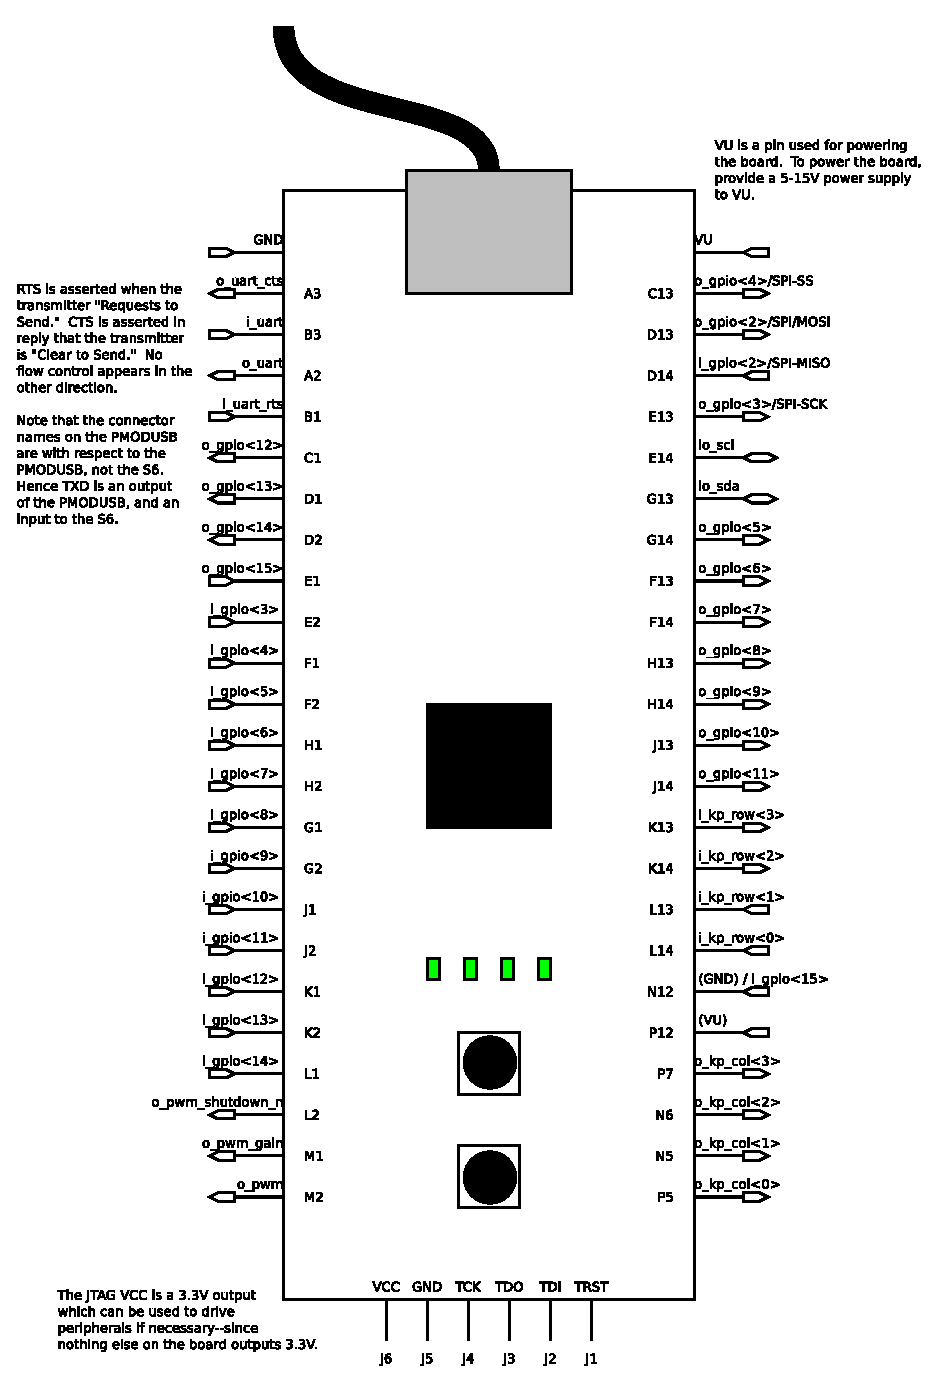
\includegraphics[height=7in]{../gfx/pinout.eps}
\caption{Physical Locations of Device I/O Ports}\label{fig:physicalio}
\end{center}\end{figure}
Although pin assignment to the actual S6~board has been rather arbitrary, there
is a touch of method to the madness.  In particular, the S6~SoC pin placement
supports placing the PMods in the configuration shown in
Fig.~\ref{fig:pmodplaces}.
\begin{figure}
\begin{center}
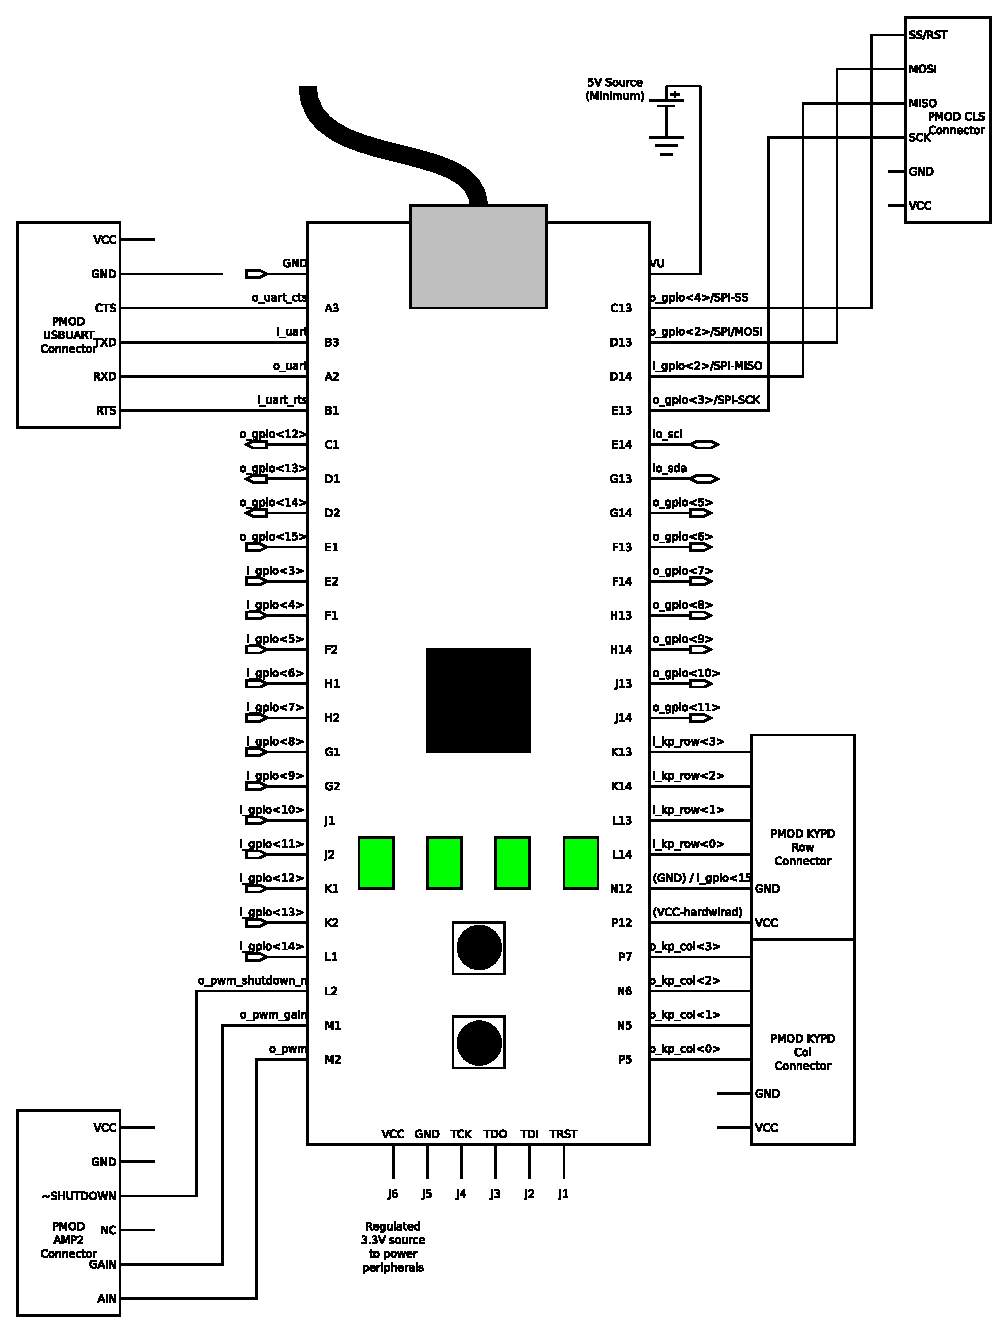
\includegraphics[height=7in]{../gfx/pmodmap.eps}
\caption{Suggested mapping of I/O ports to PMod Locations}\label{fig:pmodplaces}
\end{center}\end{figure}
From this figure you can see that I have tried to minimize the amount of
movement necessary to install any particular PMods, while also making the
greatest use of pins on board.  What may not be obvious from this picture
is that the PMod power and ground lines are all connected to power and ground
rails separate from the CMod itself.

As with any piece of open source firmware, these pin assignments are fairly
arbitrary and easy to adjust by making changes to the {\tt cmod.ucf} and
{\tt cmodtop.ucf} files.  The main difference between those two files being
the DEPP interface supported by alternate configuration, which uses
{\tt cmod.ucf}.

% Appendices
% Index
\end{document}


